\documentclass[a4wide,11pt]{article}
\usepackage[a4paper, total={6in, 8in}]{geometry}
\usepackage[dvips]{graphicx}
\usepackage{url}
\usepackage{epstopdf}
\usepackage{float}
\usepackage{csvsimple}
\usepackage{hyperref}
\usepackage{longtable}
\usepackage{fancyhdr}
\usepackage{graphicx}

\usepackage{xcolor}
\usepackage{textcomp}

\usepackage{pgfgantt}

\usepackage{enumitem}

\usepackage{array}
\newcolumntype{L}[1]{>{\raggedright\let\newline\\\arraybackslash\hspace{0pt}}m{#1}}

\pagestyle{fancy}

\hypersetup{
    colorlinks=true,
    linkcolor=blue,
    filecolor=magenta,
    urlcolor=cyan,
}
\urlstyle{same}


\definecolor{barblue}{RGB}{153,204,254}
\definecolor{groupblue}{RGB}{51,102,254}
\definecolor{linkred}{RGB}{165,0,33}
\definecolor{statusred}{RGB}{204,0,0}
\definecolor{statusgreen}{RGB}{0,153,0}
\renewcommand\sfdefault{phv}
%\renewcommand\mddefault{mc} % this causes bold, italic, .. not to be displayed
\renewcommand\bfdefault{bc}
\setganttlinklabel{s-s}{START-TO-START}
\setganttlinklabel{f-s}{FINISH-TO-START}
\setganttlinklabel{f-f}{FINISH-TO-FINISH}
\sffamily


\begin{document}

\newcommand{\greenbox}[1]{\colorbox{statusgreen!90}{\textcolor{white!90}{\textsf{\textbf{#1}}}}}
\newcommand{\graybox}[1]{\colorbox{gray!90}{\textcolor{white!90}{\textsf{\textbf{#1}}}}}
\newcommand{\lightgraybox}[1]{\colorbox{gray!40}{\textcolor{white!90}{\textsf{\textbf{#1}}}}}
\newcommand{\redbox}[1]{\colorbox{statusred}{\textcolor{white!90}{\textsf{\textbf{#1}}}}}

\title{INDIGO-DataCloud Software Quality Assurance (SQA) Report Apr-Jun 2016\\[1.5em] 
       \huge{\texttt{udocker}}\\
}

\date{} 
\maketitle

\Large
\vspace{-3em}
\begin{center}
    \graybox{\strut SQA Progress Status}\redbox{\strut NOT COMPLETE (53\% done)} \\
\end{center}

\vspace{4em}

\large
\begin{center}
\begin{tabular}{ll}
    \hyperref[sec:repository]{GitHub repository} & \greenbox{COMPLETE} \\
    \hyperref[sec:code_style]{Code style adherence} & \greenbox{COMPLETE} \\
    \hyperref[sec:unit_test]{Code coverage} & \graybox{18\%} \\ 
    %\hyperref[sec:unit_test]{Code coverage} & \begin{ganttchart}[
    %    canvas/.append style={fill=none, draw=none},
    %    hgrid style/.style={draw=none, fill=none},
    %    vgrid={*1{draw=none, fill=none}},
    %    title/.style={draw=none, fill=none},
    %    title label font=\bfseries\footnotesize,
    %    title label node/.append style={below=7pt},
    %    include title in canvas=false,
    %    bar label font=\mdseries\small\color{black!70},
    %    bar label node/.append style={left=2cm},
    %    bar/.append style={draw=none, fill=black!63},
    %    bar incomplete/.append style={fill=barblue},
    %    bar progress label font=\mdseries\footnotesize\color{black!70},
    %    bar top shift=1, bar height=0.8
    %    ]{1}{5}
    %    \ganttbar[progress=18]{}{1}{5}
    %\end{ganttchart} \vspace{0.6em}\\
    \hyperref[sec:func_int_test]{Functional/integration testing} & \graybox{IN PROGRESS - WP3} \\
    \hyperref[sec:gitbook]{GitBook documentation} & \greenbox{COMPLETE} \\
    \hyperref[sec:configuration]{Automated deployment} & \redbox{NOT COMPLETE} \\
\end{tabular}
\end{center}


\normalsize 
\newpage

\part{Task Progress}

%
% OpenProject tasks - pgfgantt
%
\hspace{-5em}
\begin{ganttchart}[
    canvas/.append style={fill=none, draw=black!5, line width=.75pt},
    hgrid style/.style={draw=black!5, line width=.75pt},
    vgrid={*1{draw=black!5, line width=.75pt}},
    today=9,
    today rule/.style={
    draw=black!64,
    dash pattern=on 3.5pt off 4.5pt,
    line width=1.5pt
    },
    today label font=\small\bfseries,
    title/.style={draw=none, fill=none},
    title label font=\bfseries\footnotesize,
    title label node/.append style={below=7pt},
    include title in canvas=false,
    bar label font=\mdseries\small\color{black!70},
    bar label node/.append style={left=2cm},
    bar/.append style={draw=none, fill=black!63},
    bar incomplete/.append style={fill=barblue},
    bar progress label font=\mdseries\footnotesize\color{black!70},
    group incomplete/.append style={fill=groupblue},
    group left shift=0,
    group right shift=0,
    group height=.5,
    group peaks tip position=0,
    group label node/.append style={left=.6cm},
    group progress label font=\bfseries\small,
    link/.style={-latex, line width=1.5pt, linkred},
    link label font=\scriptsize\bfseries,
    link label node/.append style={below left=-2pt and 0pt}
]{1}{12}
    \gantttitle[
        title label node/.append style={below left=7pt and -3pt}
    ]{WEEKS:\quad1}{1}
    \gantttitlelist{2,...,12}{1} \\
    \ganttgroup[progress=53]{\textbf{\#3641} udocker SQA FOR 1ST RELEASE}{1}{12} \\
            \ganttbar[
            progress=100,
            name=WBS1A
        ]{\textbf{\#3644} Repository synchronization}{1}{12} \\
            \ganttbar[
            progress=100,
            name=WBS1A
        ]{\textbf{\#3647} Code style specification}{1}{12} \\
            \ganttbar[
            progress=18,
            name=WBS1A
        ]{\textbf{\#3650} Unit testing coverage}{1}{12} \\
            \ganttbar[
            progress=100,
            name=WBS1A
        ]{\textbf{\#3653} Functional and integration testing coverage}{1}{12} \\
            \ganttbar[
            progress=0,
            name=WBS1A
        ]{\textbf{\#3656} Configuration management}{1}{12} \\
            \ganttbar[
            progress=50,
            name=WBS1A
        ]{\textbf{\#3659} GitBook documentation}{1}{12} \\
     [grid]
\end{ganttchart}

%\newpage

\section{Repository synchronization}
\footnotesize
\textit{Products contributing to INDIGO-DataCloud project must have their code avaiable under GitHub's \texttt{indigo-dc} organization.}
\\[0.3in]
\normalsize

\label{sec:repository}
Repository exists under \texttt{indigo-dc} GitHub organization: \vspace{0.1em} \begin{center}\url{https://github.com/indigo-dc/udocker}\end{center}


\section{Code Style}
\footnotesize
\textit{Products contributing to INDIGO-DataCloud project are expected to be adhered to a community or de-facto standard code style definition. Exceptions can be made to the selected standard. Custom style guides are accepted but nonetheless not recommended.}
\\[0.3in]
\normalsize

\label{sec:code_style}
\begin{tabular}{ll}
    Code style definition &
        \href{https://www.python.org/dev/peps/pep-0008/}{PEP 8 -- Style Guide for Python Code} \\
    Community/de-facto standard &
        \graybox{Yes} \\ 
    Exceptions & 
        \graybox{0} \\
    Richness & \graybox{\strut 73} \hspace{0.3em} \graybox{\strut Errors 63} \graybox{\strut Warnings 10} \href{http://pep8.readthedocs.io/en/latest/intro.html#error-codes}{link}\\
\end{tabular}

\subsection{Build status}
Last build status on Jenkins CI
\href{https://jenkins.indigo-datacloud.eu:8080//job/udocker-codestyle/24}{udocker-codestyle}.


 
 
\section{Unit Testing}

\label{sec:unit_test}

\begin{center}
% Trend graph (jenkins)
\textbf{Trend graph}\par\medskip
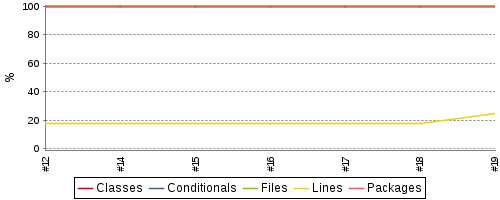
\includegraphics[scale=0.5]{/srv/metrics/reports/build/figs/graph_udocker-unittest.png}
\\
%\vspace{0.5em}
% Cobertura report (gantt chart)
%\textbf{Cobertura report}\par\medskip
\begin{ganttchart}[
    canvas/.append style={fill=none, draw=black!5, line width=.75pt},
    hgrid style/.style={draw=black!5, line width=.75pt},
    vgrid={*1{draw=black!5, line width=.75pt}},
    title/.style={draw=none, fill=none},
    %title label font=\bfseries\footnotesize,
    title label font=\normalsize,
    title label node/.append style={below=7pt},
    include title in canvas=false,
    bar label font=\mdseries\small\color{black!70},
    bar label node/.append style={left=2cm},
    bar/.append style={draw=none, fill=black!63},
    bar incomplete/.append style={fill=barblue},
    bar progress label font=\mdseries\footnotesize\color{black!70},
    group incomplete/.append style={fill=groupblue},
    group left shift=0,
    group right shift=0,
    group height=.5,
    group peaks tip position=0,
    group label node/.append style={left=.6cm},
    group progress label font=\bfseries\small,
    link/.style={-latex, line width=1.5pt, linkred},
    link label font=\scriptsize\bfseries,
    link label node/.append style={below left=-2pt and 0pt}
    ]{1}{5}
    \gantttitle{Cobertura Report}{-3} \\
    %\ganttgroup[progress=45]{Group 1}{1}{12} \\
            \ganttbar[progress=100.0]{Packages (1.0/1.0)}{1}{3} \\
            \ganttbar[progress=100.0]{Files (1.0/1.0)}{1}{3} \\
            \ganttbar[progress=100.0]{Classes (1.0/1.0)}{1}{3} \\
            \ganttbar[progress=24.989758]{Lines (610.0/2441.0)}{1}{3} \\
            \ganttbar[progress=100.0]{Conditionals (0.0/0.0)}{1}{3} \\
     [grid]
\end{ganttchart}
\end{center}
\subsection{Build status}
Last build status on Jenkins CI \href{https://jenkins.indigo-datacloud.eu:8080//job/udocker-unittest/19}{udocker-unittest}.


\section{Functional/Integration testing}

\label{sec:func_int_test}
\subsection{Observations}
\begin{enumerate}
        \item Product leader provided both functional and integration tests. WP3 is currently working on the Jenkins CI job definition.
    \end{enumerate}


\section{GitBook documentation}

\label{sec:gitbook}
Documentation available under \texttt{indigo-dc} GitBook organization: \vspace{0.1em} \begin{center}\url{https://indigo-dc.gitbooks.io/udocker/content/}\end{center} 
\subsection{Types of documentation currently provided}
\begin{center}
\graybox{\strut Readme}
\graybox{\strut User documentation}
\end{center}
\subsection{Observations}
\begin{enumerate}
        \item Task is at 50\% of progress since WP3 is waiting for the confirmation about the completeness of the documentation already provided.
    \end{enumerate}


\section{Configuration Management}
\footnotesize
\textcolor{gray!90}{\textit{Those products released by INDIGO-DataCloud project that need to be deployed by the end user must rely on a maintained open-source configuration management tool to provide an automated means to install and configure the product. The recommended tool is \texttt{Ansible}.}}
\normalsize
\\[0.1in]

\label{sec:configuration}
Product does not currently provide a automated deployment solution. 


\newpage

\appendix

\section{How to read this document}

\begin{description}[style=nextline]
\item[What are the \texttt{SQA Progress Status} possible values?] Answer: See the table below: \\[1em]
	\begin{tabular}{l L{10cm}}
		ACCEPTED & Product's SQA is compliant with the project's requirements, listed in \href{https://owncloud.indigo-datacloud.eu/index.php/s/yDklCrWjKnjutVA}{Deliverable D3.1} and \href{https://project.indigo-datacloud.eu/projects/wp3/wiki/Extensions_to_SQA}{Extensions to Software Quality Assurance} documents. \\
		NOT ACCEPTED & Product fails to fulfill one or more of the required project's SQA statements.
	\end{tabular}
\end{description}


\end{document}